\section{Aufbau}
In Abbildung \ref{fig:schemAufbau} ist der schematische Versuchsaufbau dargestellt. Verwendet wird
eine Halogenlampe, deren Wellenlängenbereich größtenteils im infraroten Bereich liegt.
\begin{figure}[H]
    \centering
    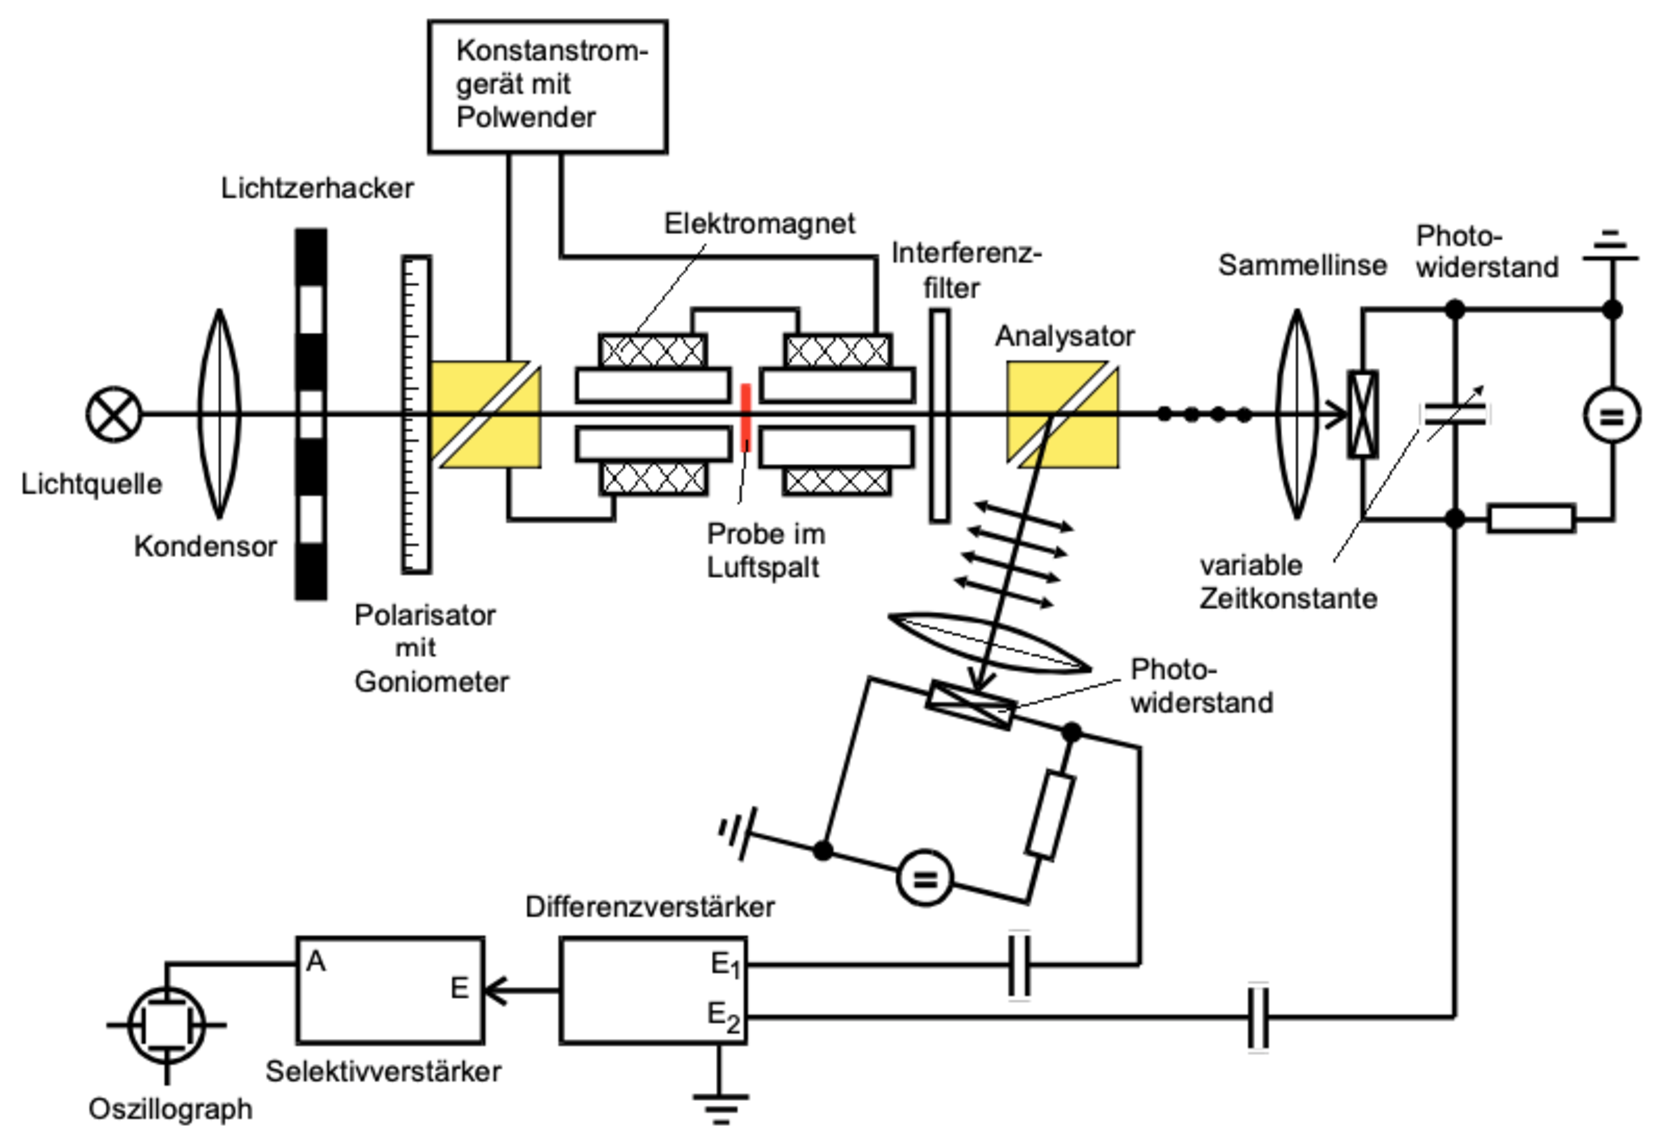
\includegraphics[width=0.8\textwidth]{images/SchemAufbau.pdf}
    \caption{Schematische Abbildung des verwendeten Versuchsaufbaus zur Bestimmung der effektiven
     Masse mithilfe des Faraday-Effekts \cite{anleitung}.}
    \label{fig:schemAufbau}
\end{figure} \noindent
Mithilfe einer Kondensorlinse wird das Licht der Halogenlampe parallelisiert bevor es den Lichtzerhacker passiert.
Daraufhin durchläft das Licht das erste Glan-Taylor-Prisma. Dieses sorgt dafür, dass auf die sich im
Elektromagneten befindliche Probe das notwendige linear polarisierte Licht trifft. 
Nachdem das Licht die Probe und die Elektromagneten durchdrungen hat, trifft es auf einen Interferenzfilter.
In diesem Versuch werden neun unterschiedliche Interferenzfilter in einem Bereich von $\SI{1.06}{\micro\meter}$ bis $\SI{2.65}{\micro\meter}$
verwendet. Durch das zweite verwendete Glan-Thompson-Prisma werden die Polarisationsanteile des 
eintreffenden Lichtes getrennt, sodass zwei Teilstrahlen entstehen. Die Intensitäten dieser werden
individuell mithilfe von Photowiderständen gemessen und in den Differenzverstärker eingespeist. Dieser 
berechnet wie der Name vermuten lässt, die Differenzen der beiden eintrefenden Signale. Dieses
Differenzsignal wird daraufhin durch den Selektivverstärker verstärkt und vom Oszilloskop visualisiert. 
Die Nutzung zweier Photowiderstände bietet eine hohe Genauigkeit. Da aufgrund der Differenzrechnung die
Bestimmung des Minimums einfacher ist. Zusätzlich ist eine Messung mit dieser Methode nicht so anfällig
gegenüber Wellenlängen- oder Intensitätsschwankungen der Halogenlampe.
Wenn stattdessen nur eine Photodiode zum Einsatz kommt, muss ein Minimum im gemessenen Signal gefunden 
werden. Oftmals würden jedoch eine Vielzahl von Drehwinkeln einem solchen Kriterium entsprechen 
und die Aufnahme der Messwerte würde ungenauer. 

\section{Durchführung}
Bevor mit der eigentlichen Messung begonnen werden kann, muss eine Justage der Versuchsapperatur durchgenommen 
werden. Dafür wird überprüft, ob die durch das zweite Glan-Thompson-Prisma entstehenden Teilstrahlen auf
die lichtempfindlichen Flächen der Photowiderstände treffen. Dafür werden die Gehäuse von den Photowiderständen
entfernt und die Position des Glan-Thompson-Prismas angepasst. Ist eine gute Position der beiden 
Teilstrahlen gegeben, wird der Lichtzerhacker eingeschaltet und die Frequenz des Selektivverstärkers auf
die Frequenz des Lichtzerhackers eingestellt. Gewüscht ist ein maximales Signal, wenn das Signal eines 
Photowiderstandes direkt auf den Selektivverstärker gegeben wird. Ist dies der Fall wird der 
Gütefaktor auf 100 geregelt. Zur letzten Überprüfung der Justage werden eine Probe, sowie ein
Interferenzfilter eingesetzt und die Signale der Photowiderstände auf die beiden Eingänge des 
Differenzverstärkers gelegt. Beim Durchgehen eines großen Winkelbereichs am Polarisator sollte im Abstand von ca. 
$\SI{90}{\degree}$ periodisch ein minimales Signal zu beobachten sein. Ist dies nicht der Fall, sollte 
die Justage erneut vorgenommen werden. Ein besonderes Augenmerk sollte dabei auf dem Konstrast liegen. 
Idealerweise verschwindet einer der Teilstrahlen, während der Andere eine maximale Intensität aufweist. \\
\\
Nachdem die Justage erfolgreich abgeschlossen ist, wird mit der eigentlichen Messung begonnen. Zunächst 
wird die hochreine Galium-Arsenit Probe in den Versuchsaufbau eingefügt. Mithilfe des Oszilloskops 
wird der Polarisationswinkel gesucht bei dem sich das minimale Signal einstellt. Dieser wird notiert und
daraufhin das Magnetfeld umgepolt und der Vorgang wiederholt. Auf diese Weise wird die Probe im Zusammenspiel
mit den neun verschiedenen Interferenzfiltern untersucht. \\
Analog dazu werden zwei n-dotierte Galium-Arsenit Proben untersucht. Dabei handelt es sich bei Probe 1 
um eine $\SI{1.36}{\milli\meter}$ dicke Probe mit einer Ladungsträgerdichte von
$\SI{1.2e18}{\cubic\centi\meter}$. Die zweite Probe ist $\SI{1.296}{\milli\meter}$ dick und weist eine 
Ladungsträgerdichte von $\SI{2,8e18}{\cubic\centi\meter}$ auf. \\
Im letzten Schritt der Durchführung wird das vorherrschende Magnetfeld in der Nähe des im Elektromagneten 
vorhandenen Luftspaltes mithilfe einer Hallsonde ausgemessen und die Werte notiert.